% !TEX root = ../paper.tex
%http://sphweb.bumc.bu.edu/otlt/MPH-Modules/BS/BS704_HypothesisTesting-ANOVA/BS704_HypothesisTesting-Anova_print.html
\section{Results}\label{sec:results}
Some data points needed to be removed from the experiments, in order to gain a clearer understanding of the experimental outcomes. 

From \studyone: \target, we started with a total of 7344 attempts.
176 were removed because of system errors, where the system wrongly activated a technique attempt even though the user did not intend to do so.
Another 406 attempts were removed as outliers using the Outlier Labeling method described by Hoaglin and Iglewicz in Resistant Rules for Outlier Labeling \cite{Hoaglin:1987}.
This gave us a total of 6762 attempts for \studyone.

From \studytwo: \accuracy, we started with a total of 4752 attempts.
111 attempts were removed due to system errors. 
Another 138 attempts were removed with the same Outlier Labeling method used above.
This gave us a total of 4503 attempts for \studytwo.

\Cref{tab:numberOfAttempts} shows the final number of attempts each technique had in the two different experiments

\begin{table}[H]
	\centering
	\textbf{Number of attempts}\\[4pt]
	\begin{adjustbox}{width=\columnwidth}
		{
			\def\arraystretch{1.5}
			\begin{tabular}{c c c c c}
				& \multicolumn{4}{c}{\textbf{STUDY ONE}} \\
				\cline{2-5}
				& \textbf{Grab} & \textbf{Swipe} & \textbf{Throw} & \textbf{Tilt} \\ \hline
				\textbf{Push} & 830 & 835 & 814 & 862 \\ \hline
				\textbf{Pull} & 784 & 893 & 867 & 877 \\ \hline
			\end{tabular}
		}
		{
			\def\arraystretch{1.5}
			\begin{tabular}{c c c c c}
				& \multicolumn{4}{c}{\textbf{STUDY TWO}} \\
				\cline{2-5}
				& \textbf{Grab} & \textbf{Swipe} & \textbf{Throw} & \textbf{Tilt} \\ \hline
				\textbf{Push} & 551 & 576 & 561 & 582 \\ \hline
				\textbf{Pull} & 533 & 576 & 569 & 555 \\ \hline
			\end{tabular}
		}
	\end{adjustbox}
	\caption{Number of attempts for each technique in each study}
	\label{tab:numberOfAttempts}
\end{table}

\subsection{STUDY ONE: Success rate}
Here we present results relating to whether or not the user hit the target, which we will be referring to as effectiveness when discussing the results in \studyone. 

To see whether or not each technique had an effect on the success rate of each attempt, and was not just noise, we performed a Pearsons Chi-Square test on both data sets. 
For the \push techniques, $X(3)=121.950$, $p<0.001$, and for the \pull techniques we got $X(3)=438.473$, $p<0.001$. 
This means that both \push and \pull techniques had a significant effect on the success rate of each attempt, and was not purely coincidental. 
\Cref{tab:successRate} shows the success rate for each of the techniques. 

\begin{table}[H]
	\centering
	\def\arraystretch{1.5}
		\begin{tabular}{c c c c c}
			& \multicolumn{4}{c}{\textbf{Hit Success Means}} \\
			\cline{2-5}
			& \textbf{Grab} & \textbf{Swipe} & \textbf{Throw} & \textbf{Tilt} \\ \hline
			\textbf{Push} & 95.9\% & 96\% & 93.2\% & 83.3\% \\ \hline
			\textbf{Pull} & 94\% & 97.5\% & 96.7\% & 71.8\% \\ \hline
		\end{tabular}
	\caption{Success rate for each technique in \studyone}
	\label{tab:successRate}
\end{table}

\subsection{STUDY ONE: Time taken}
Here, we present results in regards to how long each user took in performing each technique in \studyone. 
When discussing these results, we will be referring to a technique's efficiency.

We performed a linear mixed effects model analysis on the data to see how time was affected by the different aspects of our experiment. 
We found out that a successful hit had no effect on the time each user took per attempt ($F_{1,6706.785} = 2.283, p = 0.131$), and neither had the direction of the technique ($F_{1,6695.822} = 1.952, p = 0.162$). 
However, the target size ($F_{1,6695.228} = 91.634, p < 0.001$) and the technique  ($F_{1,6695.228} = 91.634, p < 0.001$) did have significant effects on the time taken per attempt. 
We performed a post-hoc LSD pairwise comparison on the techniques to see how each technique differed from one another and found that all techniques were significantly different $(p<0.001)$ from each other. 

We also found that there were other interactions between the variables that were affecting the time for each attempt differently. 
$Direction \times Technique$  ($F_{3,6694.657} = 52.272, p < 0.001$), $Effectiveness \times Technique$  ($F_{3,6696.169} = 5.227, p < 0.001$) and finally $Effectiveness \times Direction \times Technique$  ($F_{3,6696.038} = 10.235, p < 0.001$) all showed to be significant interactions. 
We then ran another post-hoc LSD pairwise test between successful and failed techniques for each technique and direction to see where that significance was. 
The only significantly different pair was between the \grab \push and \grab \pull techniques $(p < 0.001)$.

Below you can find the means for each technique and direction in \cref{fig:efficiencyGraph}

\begin{figure}[H]{
	\centering
	\textbf{Efficiency}\\[4pt]
	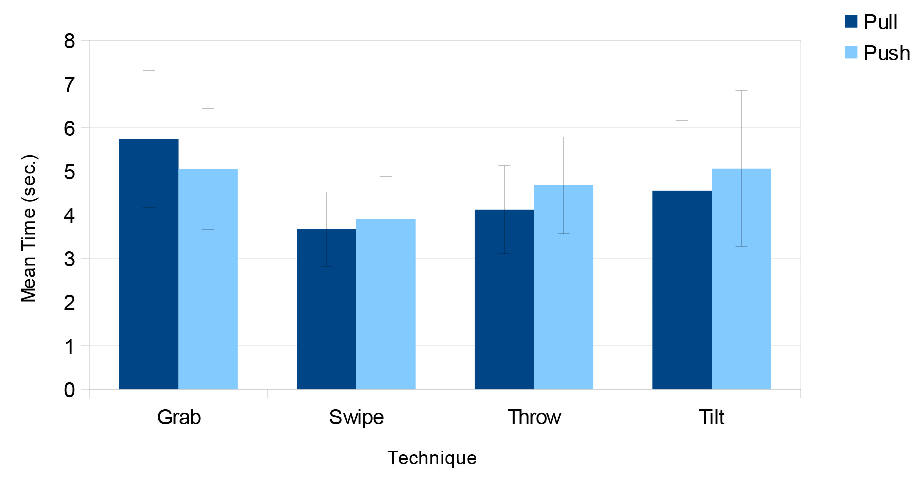
\includegraphics[width = 1\columnwidth ]{images/time_graph.pdf}} 
	\caption{
		Mean and standard deviation for each technique in regards to efficiency.
	}
	\label{fig:efficiencyGraph}
\end{figure}

\subsection{STUDY TWO: Distance from target}
Here we present the results in regards to how far away from the center of the target (in pixels) each user was when performing the technique in \studytwo. 
This is referred to as a techniques accuracy when we discuss the results. 

We performed a linear mixed effects model analysis on the data to see if each technique had a significant effect on the accuracy of each attempt. 

We found that each technique did have a significant effect on accuracy ($F_{3,4458.26}=193.869, p<0.001$).
We also found that the target size also had an effect on accuracy ($F_{1,4462.203}=100.016, p<0.001$).
The direction of each technique did not have an effect on accuracy though ($F_{1,4457.244}=0.694, p=0.405$). 
We then performed a post-hoc LSD pairwise comparison between the techniques to see were the differences lay, and found that all techniques were significantly different from each other ($p<0.003$ for all).

We also found that the interaction between direction and technique also had a significant effect on the accuracy of each attempt($F_{3,4457.354}=8.882, p<0.001$). 
We then performed another LSD pairwise comparison of each technique with the same direction. 
We found that the only pair that was not significantly different from each other was between the \pull versions of the \grab and \throw techniques. ($p=0.508$). 
All others were significantly different from one another ($p<0.004$). 

Below you can see the mean for each technique and direction in \cref{fig:accuracyGraph}
\begin{figure}[H]{
	\centering
	\textbf{Accuracy}\\[4pt]
	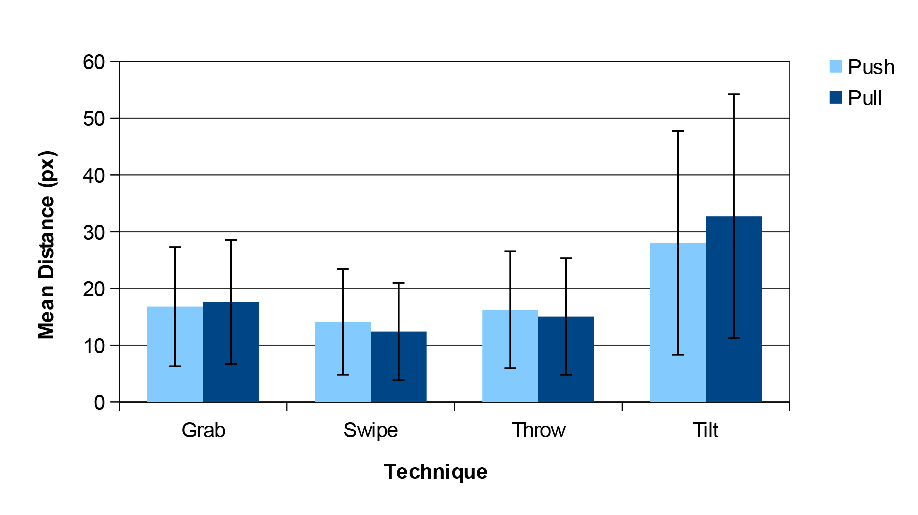
\includegraphics[width = 1\columnwidth ]{images/distance_graph.pdf}} 
	\caption{
		Mean and standard deviation for each technique in regards to accuracy.
	}
	\label{fig:accuracyGraph}
\end{figure}




